\documentclass[a4paper,11pt]{article}

\usepackage{lipsum}
\usepackage[english]{babel}
\usepackage[margin=20mm]{geometry}
\usepackage{amsmath}
\usepackage{graphicx}
\usepackage{hyperref}

\title{Computer Graphics OpenGL Coursework}
\date{\today}
\author{James King}

\begin{document}
\maketitle

\section{Application Overview}
The application models a lone motor boat traversing an infinite and empty ocean, and simulates some simple water dynamics such as the wake left behind the boat as it moves. The boat may be controlled by the user, and a virtual camera may be oriented to look in any direction. It is also possible to toggle between a first-person view from within the boat to a third-person chase camera.

The implementation is written in the C$\sharp$ programming language on the .NET Framework v4.0, using the freely available OpenTK library to interface with OpenGL. I have had some prior experience with OpenGL, so my main intention for this project was to explore some graphical techniques that I hadn't previously used. These techniques include parsing .obj files, water shaders, environment mapping, and frame buffer objects. Also, the implementation would aim to include no deprecated OpenGL calls from older version of the library, and would be entirely using the shader program rendering model.

\section{Assessment Criteria Catchment}
\subsection{Model Structures}
\subsubsection{Ship Model}
The ship model was created using the free 3D modelling application Blender, and exported as a Wavefront OBJ (.obj) file which could then be imported into the application using a parser written by myself. The vertex normals have been smoothed by the modelling application so that they are the average normals of all faces connected to that vertex, to improve light shading effects.

The model is split into several groups, which are referred to as `Face Groups' within the application. The purpose of the groups is to allow different parts of the ship to have different material effects; and in the case of the outboard motor and propeller, to have a different transformation applied before rendering. The groups that the ship has been divided into are inner hull, outer hull, trim, motor, tiller and propeller. There is also one additional face group in the model; a plane covering the top of the ship. This `depth clip plane' is used in a mechanism that stops water from being drawn inside the ship, which will be explained later. All the face group vertex data is stored in a single vertex buffer object, with pointers to the start index and length of each group so that they may be rendered individually.

\subsubsection{Sea Model}
Unlike the ship model, the sea model is generated procedurally when the application launches. My implementation for drawing the sea uses a vertex shader looking up a displacement map to determine the height of the sea at each point on the surface, so all the model needs to be is a flat grid of quads. Because the details of the sea are encoded in a series of textures, the sea model itself can remain almost stationary in eye-space, with the exception being that it must pitch when the camera looks up or down in order to remain on a fixed plane in world-space. While generating the mesh, I have implemented a level of detail (LOD) reduction effect for quads further from the camera, and also culled quads that would be outside the camera's field of view.

\subsection{Program Implementation}
\subsubsection{Graphics Canvas and Light Settings}
I have made an effort to cleanly abstract most low-level OpenGL calls in such a way as to minimise code duplication and improve readability. For example, I have written wrapper classes for frame buffer objects, vertex buffer objects, textures and shader programs. Light is implemented in the shader which draws the boat through a diffuse and specular model, using a global light direction contained within a structure holding information about the scene. The water shader also has a slight diffuse effect, but the main material effect is a reflection of the sky environment map. The sky is a simple environment mapped cube surrounding the camera in a fixed position in eye-space.

\subsubsection{Drawing of the Ship Model}
The ship is drawn with two different textures for different parts, and uses the global light direction for a diffuse and specular lighting effect which also varies in magnitude for different parts. A previous problem was that water would be drawn inside the ship when the main water plane was rendered, which has been fixed by drawing an invisible plane across the top of the ship that still writes to the depth buffer, therefore hiding any water drawn behind it.

\subsubsection{Drawing of the Sea Model}
The sea is the most complex part of the application. Along with the static surface quad mesh, the sea uses three textures to encode wave height, wave velocity, and the amount of spray on the surface. The sea is modelled as a large grid of columns, with virtual springs between the top of each column. When some columns are depressed (for example by the ship traversing across them) they accelerate upwards to try and match the average height of their neighbours, and the neighbours will accelerate downwards also. This, when simulated every update, causes ripples in the surface of the water. The spray texture slowly dissipates any high concentrations of spray, and will increase the amount of spray at a point if the velocity texture has a very high magnitude. The simulation is implemented using a series of shaders outputting to frame buffer objects, which write to the three water textures. Originally this was all done on the CPU without frame buffer objects, but offsetting the work to the GPU has allowed much more detailed water textures to be used.

When rendering, the height texture is used as a displacement map in the water vertex shader to offset the vertical position of each vertex in the mesh. The height texture is also used in the fragment shader to find the surface normal at each fragment, which is then used in the sky reflection effect. The spray is drawn when the spray texture value at each fragment exceeds a threshold, and is modulated by a small noise texture that is generated when the program starts.

\subsubsection{Ship Movement}
The ship can traverse the surface of the water, with some basic physics reacting to the state of the surface it is touching. The outboard motor and tiller pivot on the spot relative to the ship's position, and the propeller spins independently with a fixed position relative to the rudder.

\subsection{Interaction}
The boat may be accelerated forwards with the W key, backwards with S key, and rotate left and right with the A and D keys respectively. The camera may be rotated with the mouse (the window must be clicked on first to enable mouse look), and the camera may be toggled between first person and chase cam with V. It is also possible to view a wireframe version of the scene with L, and to hide the ship with B. The mouse may be detached with the Esc key, and fullscreen toggled with Alt+Enter.

\subsection{Robustness}
Assuming the application is executed on a system with a graphics card capable of the various OpenGL features used, the application runs consistently and without error. It has been tested on Windows and Linux, and on NVidia and ATI graphics cards successfully.

\section{Limitations of the Design}
The application relies on some fairly modern rendering techniques, so a recent graphics card is needed to see all the program has to offer. Also, the method used to simulate a wake behind the boat uses textures of finite size which wrap across their edges. It is therefore possible to see your own wake ahead of you when travelling fast enough in one direction. There currently aren't any options to change the rendering quality of various aspects of the program, so the performance can't yet be increased on slower machines.

\section{Setup and Use}
All files required to run the application are contained within the archive, although the .NET Framework v4.0 (or a recent version of Mono) is needed. To run, extract all files in the archive to a directory, then execute the .exe file. Also, as previously mentioned, a fairly recent graphics card is essential.

\section{Opportunities for Improvement}
Originally, the goal was to make a simple boat racing game where the player would attempt to navigate around a series of buoys along a route. Also, I was hoping to implement islands, but chose instead to focus on improving the water quality. Fixing the aforementioned problem with seeing your own wake repeat and the addition of customisable options are also features I would implement given enough time. Also, I would have liked to have comprehensively commented all of the source code, but ran out of time after commenting a few core files.

\section{References}
\subsection{Open Toolkit Library}
Used for the OpenGL bindings, context creation and matrix helper functions

\url{http://www.opentk.com/}

\subsection{Stormy Days Sky Environment Map}
By Jockum `hipshot' Skoglund

\url{http://forums.epicgames.com/threads/506748-My-skies-and-and-cliff-textures-(large-images}

\subsection{Plank Texture}
Photographed and edited by Dmitriy Chugai

\url{http://texturelib.com/texture/?path=/Textures/wood/planks+new/wood_planks_new_0034}

\subsection{Fiberglass Texture}
Provided by CGTextures.com

\url{http://www.cgtextures.com/texview.php?id=9707&PHPSESSID=7pk7t90or58pkeh3gnn73k1601}

\newpage
\section{Screen Shots}
\begin{figure}[h!]
\centering
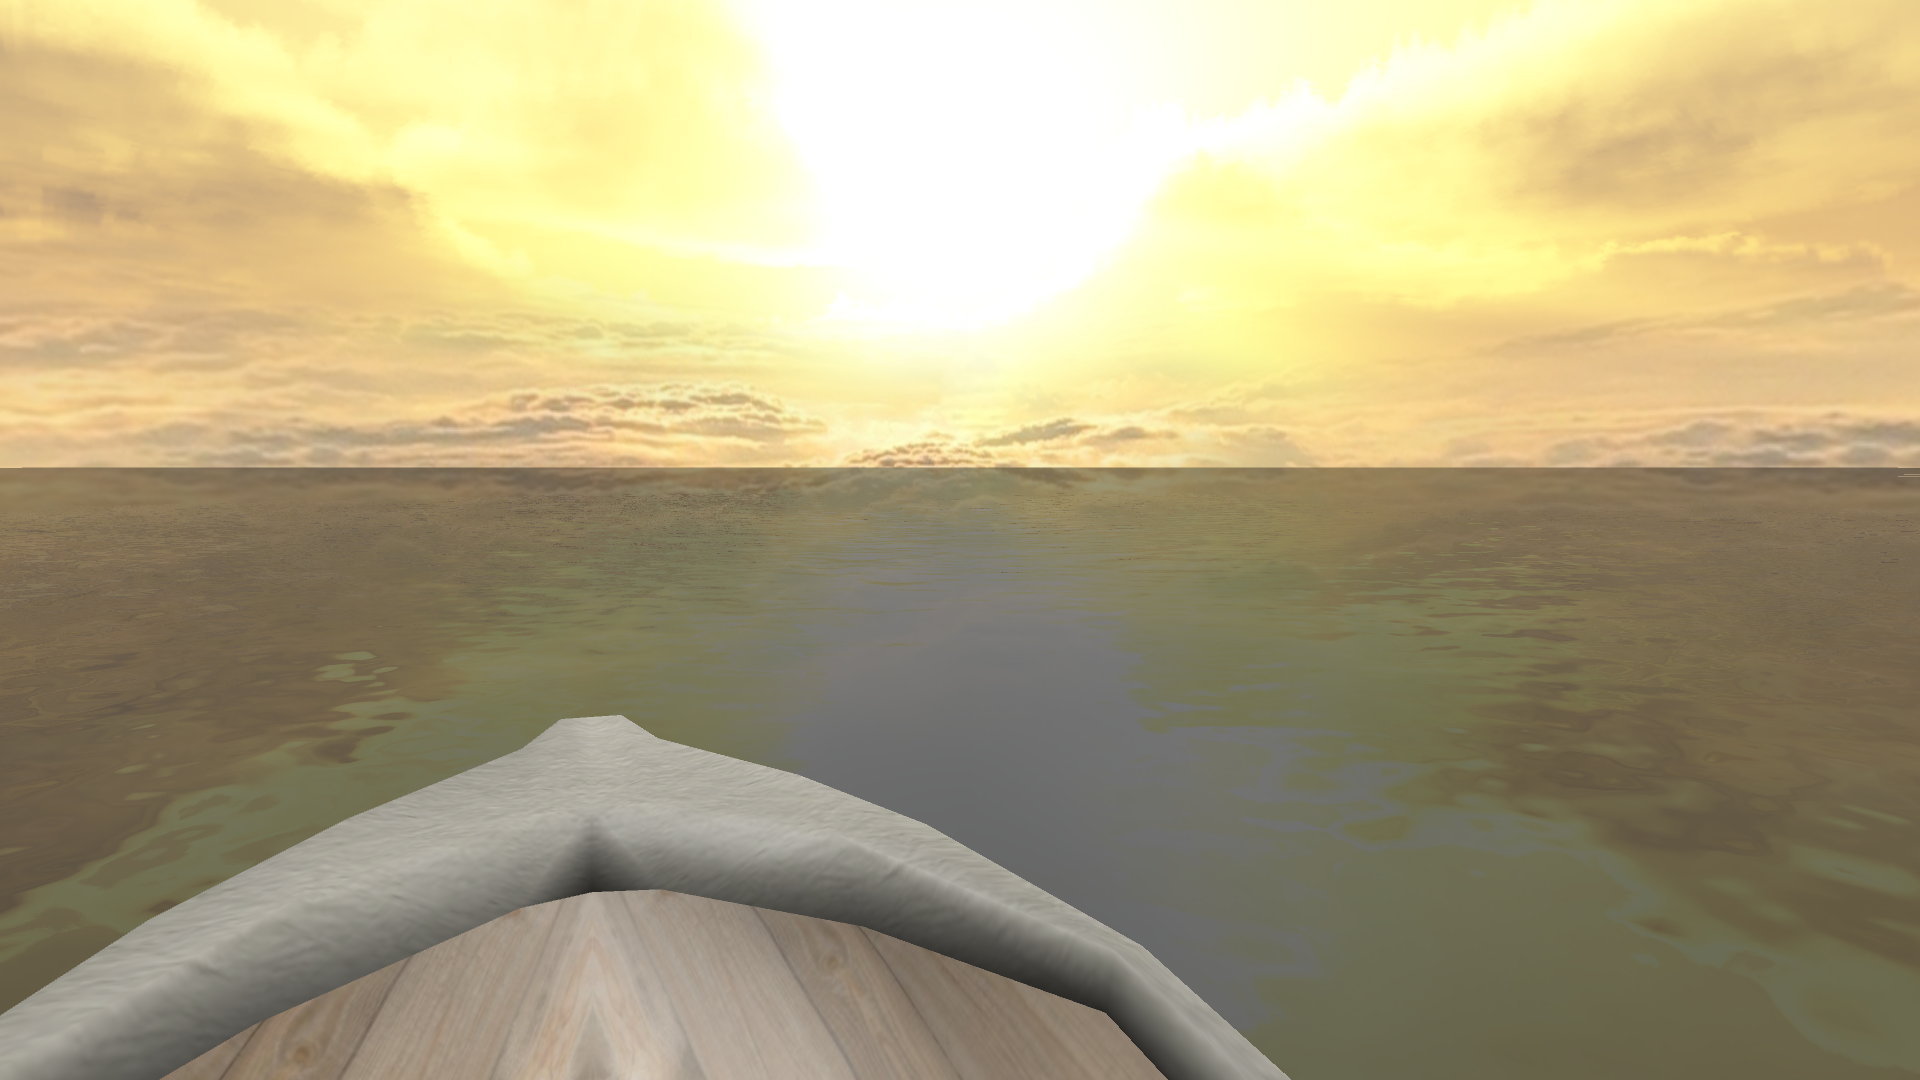
\includegraphics[width=\textwidth]{screen1.png}
\caption{First person view, showing the reflective water shader and sky}
\end{figure}

\begin{figure}[h!]
\centering
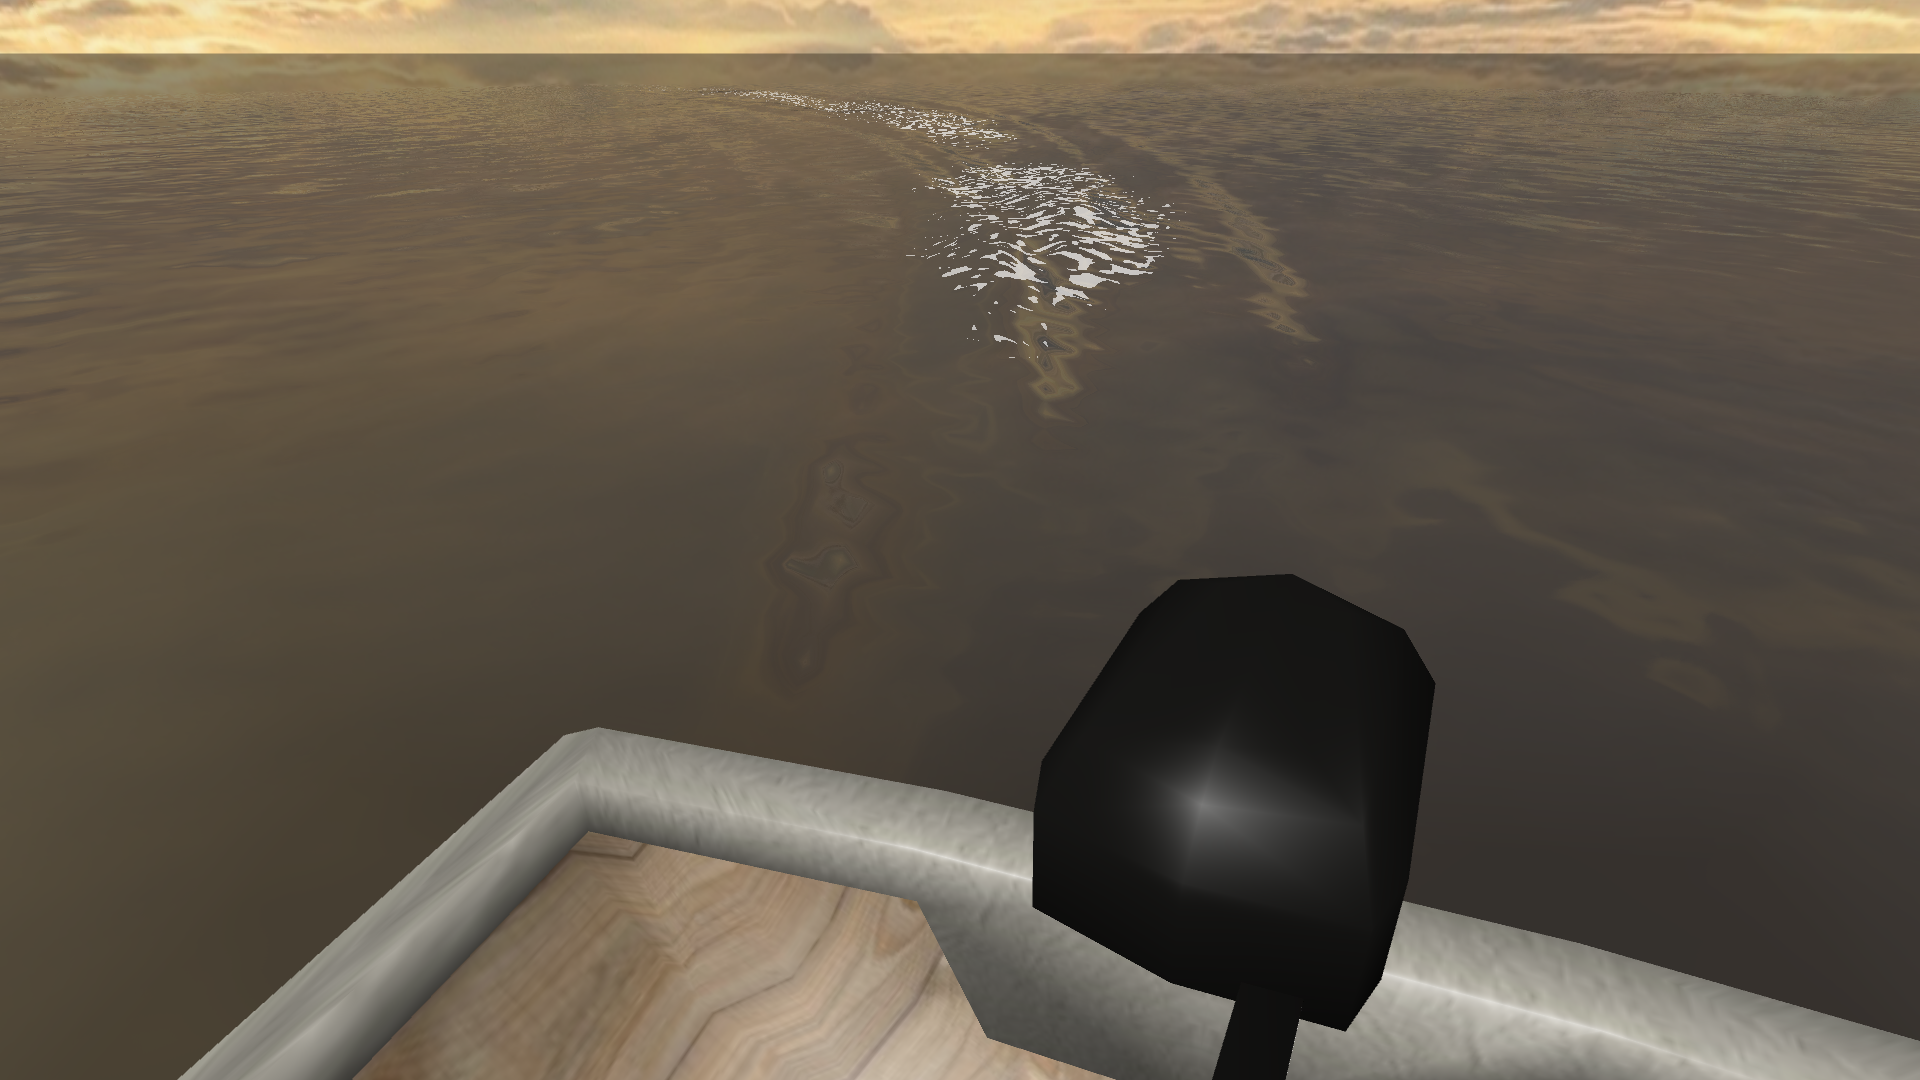
\includegraphics[width=\textwidth]{screen4.png}
\caption{First person view, showing the wake behind the boat}
\end{figure}

\begin{figure}[h!]
\centering
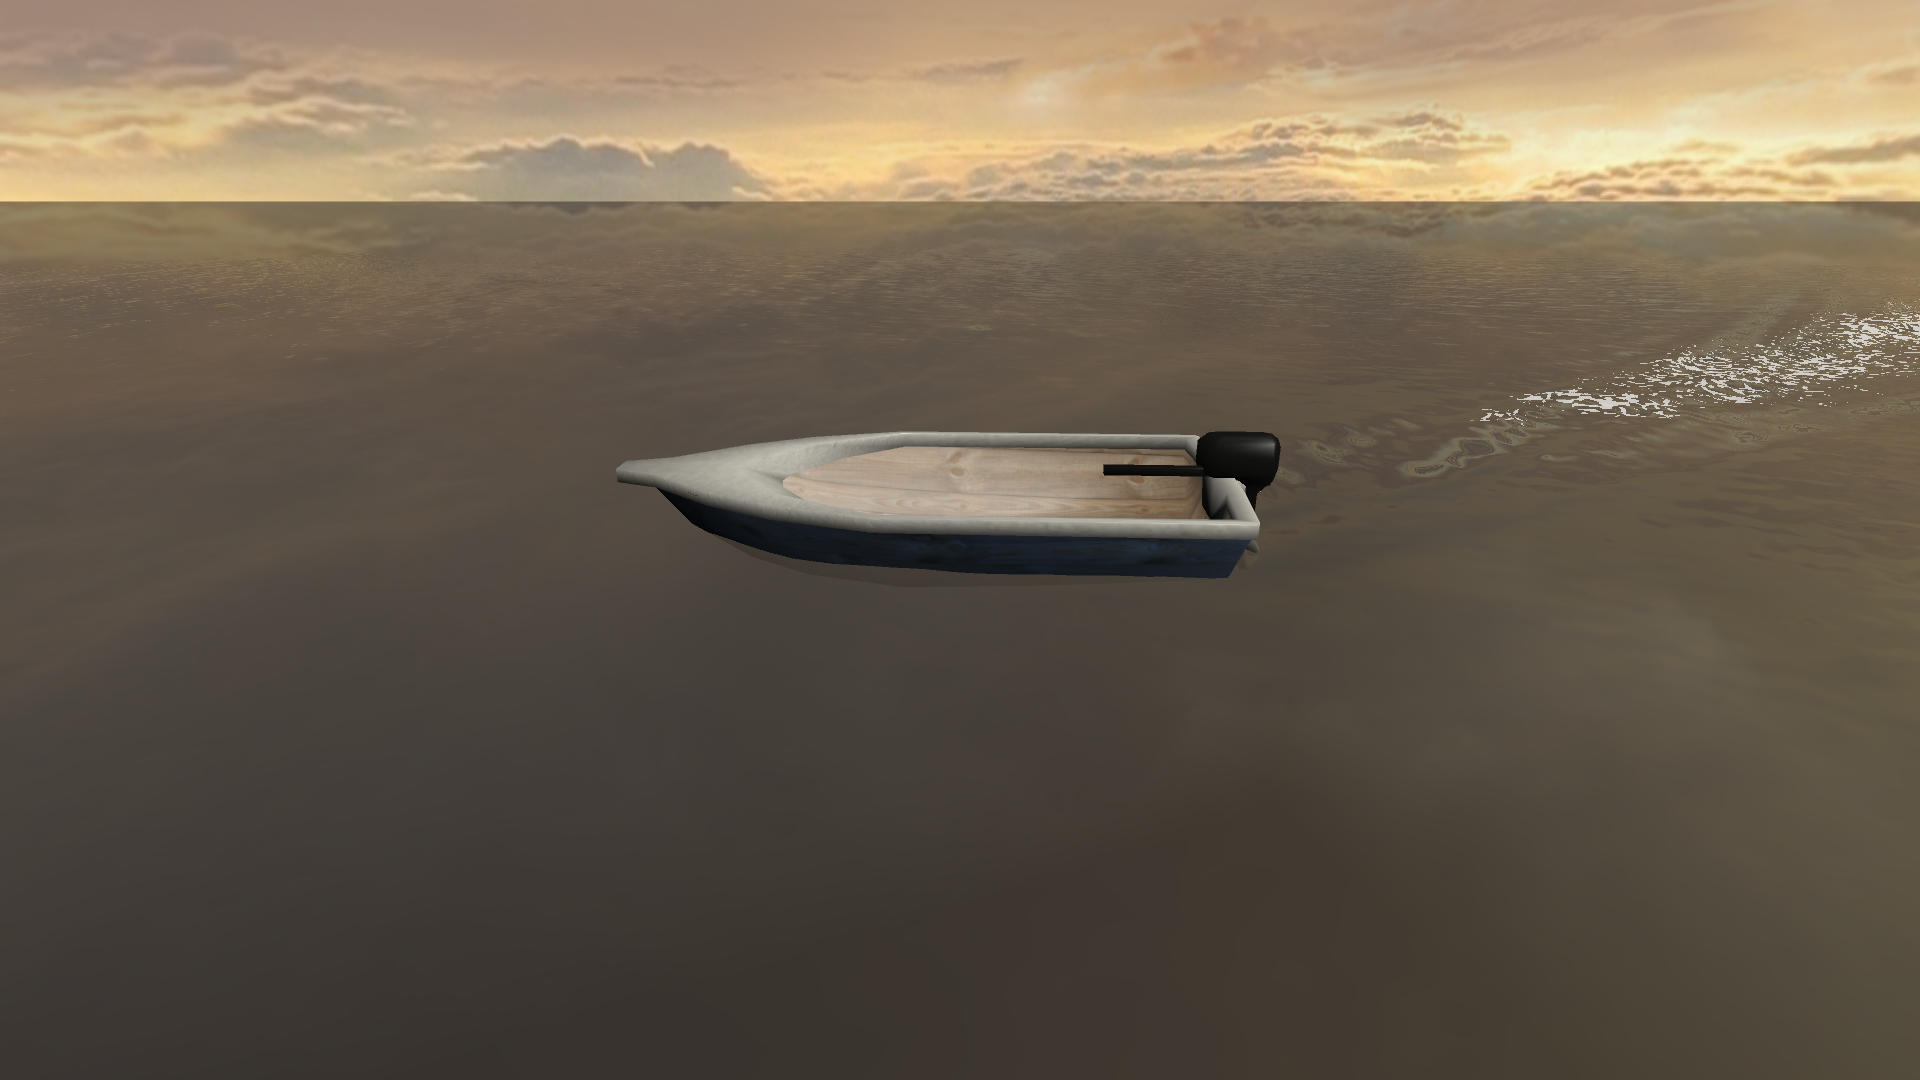
\includegraphics[width=\textwidth]{screen2.png}
\caption{The whole boat in third person view, along with its dynamic wake}
\end{figure}

\begin{figure}[h!]
\centering
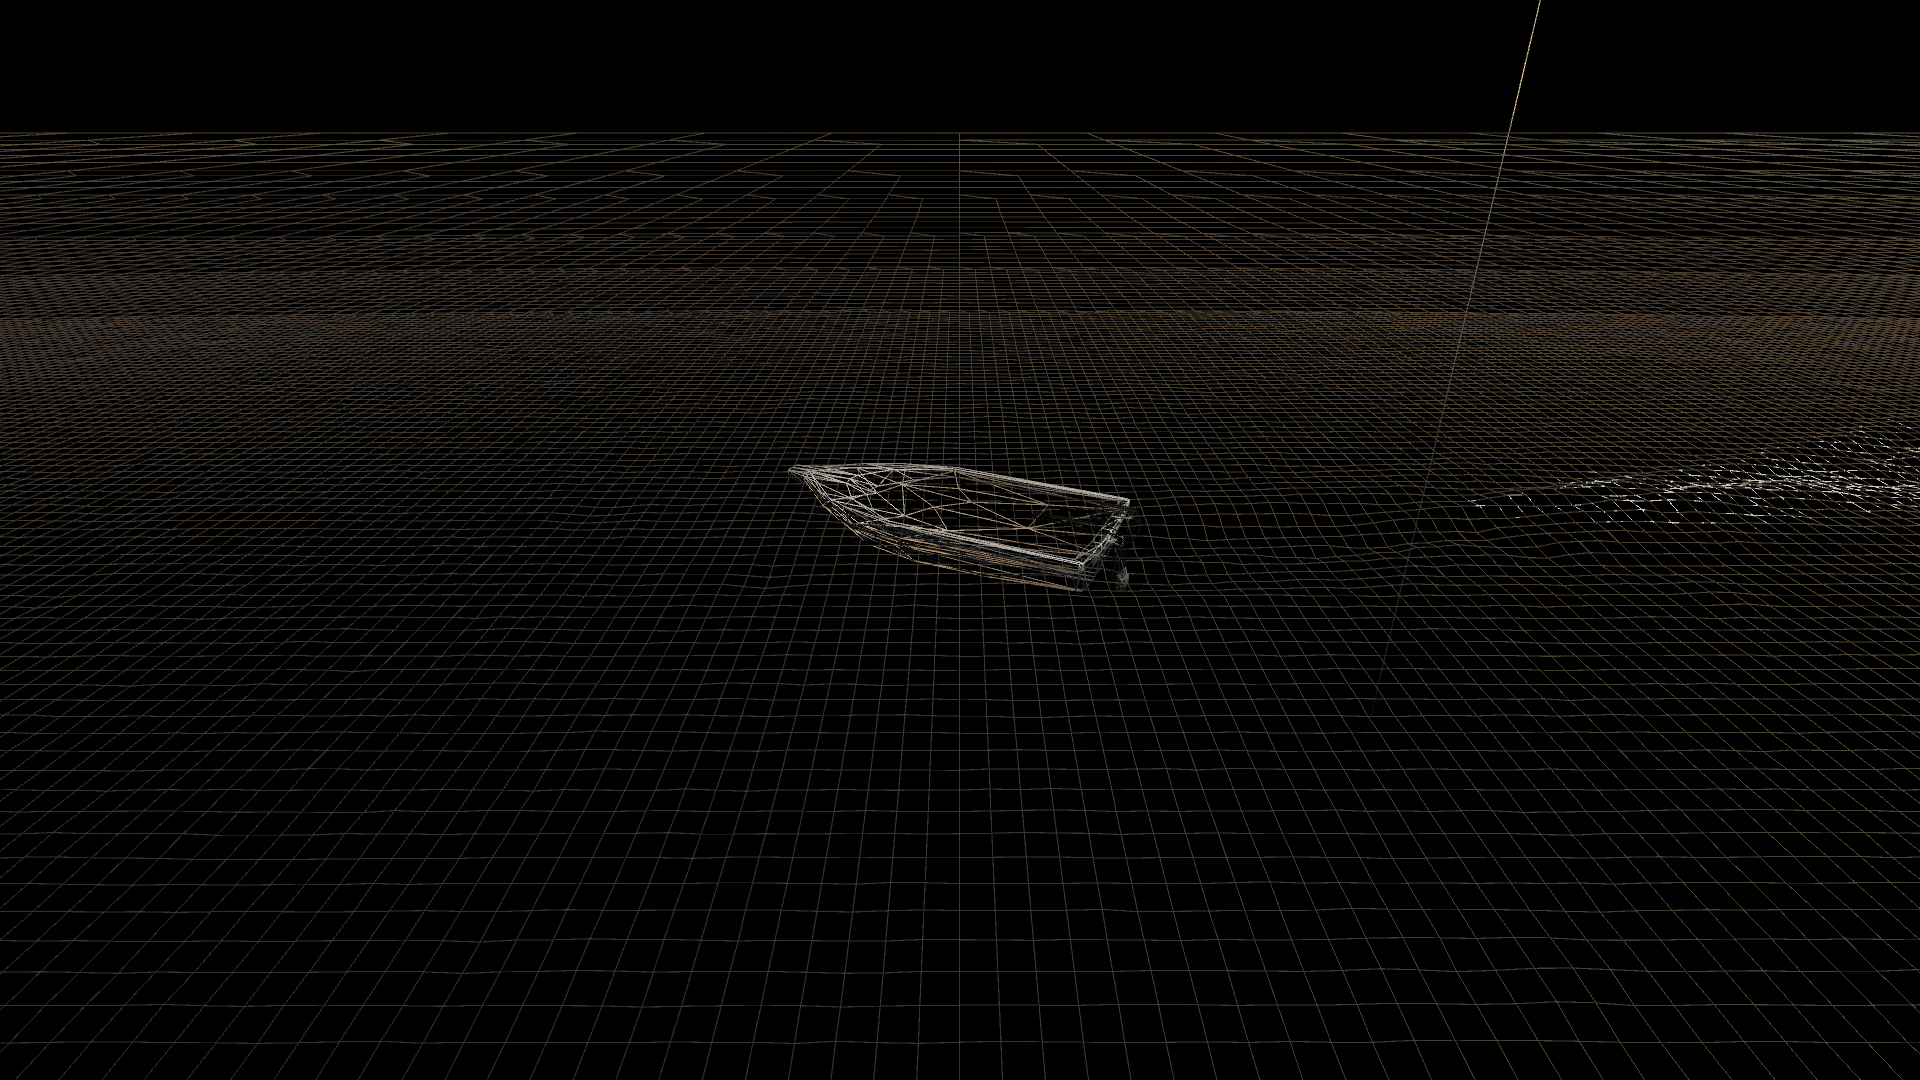
\includegraphics[width=\textwidth]{screen3.png}
\caption{Wireframe view showing the water mesh structure}
\end{figure}
\end{document}
